\section{Methodology}
\label{sec:methodology}
	
	\subsection{Measured Data}
	\label{ssec:measured-data}
	
		As a single spectrum contains overlapping information, it is necessary to determine both relevant wavelengths and the respective parameters to apply NIRS to practical problems.
		To select wavelengths and determine parameters we use a training set, which contains $p^\m{(SOC)},p^\m{(N)},\m{pH}$ and wave reflectances of 319 wavelengths ranging from $1400 \unit{nm}$ to $2672 \unit{nm}$ by steps of $4 \unit{nm}$ for 533 samples \cite{don:a}.

		We define $\Lambda$ as the set of all measured wavelengths. The reflectance $\varrho(\lambda)$ of a sample at a wavelength $\lambda \in \Lambda$ is recorded as
		\[
			-\lg \varrho(\lambda) = -\frac{\ln \varrho(\lambda)}{\ln 10}
		\]
		Figure \ref{fig:soil-spec-rnd} shows six randomly chosen soil spectra in a diagram.
		\begin{figure*}
			\centering
			% GNUPLOT: LaTeX picture with Postscript
\begingroup
  \makeatletter
  \providecommand\color[2][]{%
    \GenericError{(gnuplot) \space\space\space\@spaces}{%
      Package color not loaded in conjunction with
      terminal option `colourtext'%
    }{See the gnuplot documentation for explanation.%
    }{Either use 'blacktext' in gnuplot or load the package
      color.sty in LaTeX.}%
    \renewcommand\color[2][]{}%
  }%
  \providecommand\includegraphics[2][]{%
    \GenericError{(gnuplot) \space\space\space\@spaces}{%
      Package graphicx or graphics not loaded%
    }{See the gnuplot documentation for explanation.%
    }{The gnuplot epslatex terminal needs graphicx.sty or graphics.sty.}%
    \renewcommand\includegraphics[2][]{}%
  }%
  \providecommand\rotatebox[2]{#2}%
  \@ifundefined{ifGPcolor}{%
    \newif\ifGPcolor
    \GPcolorfalse
  }{}%
  \@ifundefined{ifGPblacktext}{%
    \newif\ifGPblacktext
    \GPblacktexttrue
  }{}%
  % define a \g@addto@macro without @ in the name:
  \let\gplgaddtomacro\g@addto@macro
  % define empty templates for all commands taking text:
  \gdef\gplbacktext{}%
  \gdef\gplfronttext{}%
  \makeatother
  \ifGPblacktext
    % no textcolor at all
    \def\colorrgb#1{}%
    \def\colorgray#1{}%
  \else
    % gray or color?
    \ifGPcolor
      \def\colorrgb#1{\color[rgb]{#1}}%
      \def\colorgray#1{\color[gray]{#1}}%
      \expandafter\def\csname LTw\endcsname{\color{white}}%
      \expandafter\def\csname LTb\endcsname{\color{black}}%
      \expandafter\def\csname LTa\endcsname{\color{black}}%
      \expandafter\def\csname LT0\endcsname{\color[rgb]{1,0,0}}%
      \expandafter\def\csname LT1\endcsname{\color[rgb]{0,1,0}}%
      \expandafter\def\csname LT2\endcsname{\color[rgb]{0,0,1}}%
      \expandafter\def\csname LT3\endcsname{\color[rgb]{1,0,1}}%
      \expandafter\def\csname LT4\endcsname{\color[rgb]{0,1,1}}%
      \expandafter\def\csname LT5\endcsname{\color[rgb]{1,1,0}}%
      \expandafter\def\csname LT6\endcsname{\color[rgb]{0,0,0}}%
      \expandafter\def\csname LT7\endcsname{\color[rgb]{1,0.3,0}}%
      \expandafter\def\csname LT8\endcsname{\color[rgb]{0.5,0.5,0.5}}%
    \else
      % gray
      \def\colorrgb#1{\color{black}}%
      \def\colorgray#1{\color[gray]{#1}}%
      \expandafter\def\csname LTw\endcsname{\color{white}}%
      \expandafter\def\csname LTb\endcsname{\color{black}}%
      \expandafter\def\csname LTa\endcsname{\color{black}}%
      \expandafter\def\csname LT0\endcsname{\color{black}}%
      \expandafter\def\csname LT1\endcsname{\color{black}}%
      \expandafter\def\csname LT2\endcsname{\color{black}}%
      \expandafter\def\csname LT3\endcsname{\color{black}}%
      \expandafter\def\csname LT4\endcsname{\color{black}}%
      \expandafter\def\csname LT5\endcsname{\color{black}}%
      \expandafter\def\csname LT6\endcsname{\color{black}}%
      \expandafter\def\csname LT7\endcsname{\color{black}}%
      \expandafter\def\csname LT8\endcsname{\color{black}}%
    \fi
  \fi
  \setlength{\unitlength}{0.0500bp}%
  \begin{picture}(7936.00,3400.00)%
    \gplgaddtomacro\gplbacktext{%
      \csname LTb\endcsname%
      \put(1078,704){\makebox(0,0)[r]{\strut{} 0.3}}%
      \put(1078,1190){\makebox(0,0)[r]{\strut{} 0.35}}%
      \put(1078,1676){\makebox(0,0)[r]{\strut{} 0.4}}%
      \put(1078,2163){\makebox(0,0)[r]{\strut{} 0.45}}%
      \put(1078,2649){\makebox(0,0)[r]{\strut{} 0.5}}%
      \put(1078,3135){\makebox(0,0)[r]{\strut{} 0.55}}%
      \put(1353,484){\makebox(0,0){\strut{} 1400}}%
      \put(2304,484){\makebox(0,0){\strut{} 1600}}%
      \put(3256,484){\makebox(0,0){\strut{} 1800}}%
      \put(4208,484){\makebox(0,0){\strut{} 2000}}%
      \put(5160,484){\makebox(0,0){\strut{} 2200}}%
      \put(6111,484){\makebox(0,0){\strut{} 2400}}%
      \put(7063,484){\makebox(0,0){\strut{} 2600}}%
      \put(176,1919){\rotatebox{-270}{\makebox(0,0){\strut{}$-\lg \varrho(\lambda)$}}}%
      \put(4374,154){\makebox(0,0){\strut{}$\lambda \ [\m{nm}]$}}%
    }%
    \gplgaddtomacro\gplfronttext{%
    }%
    \gplbacktext
    \put(0,0){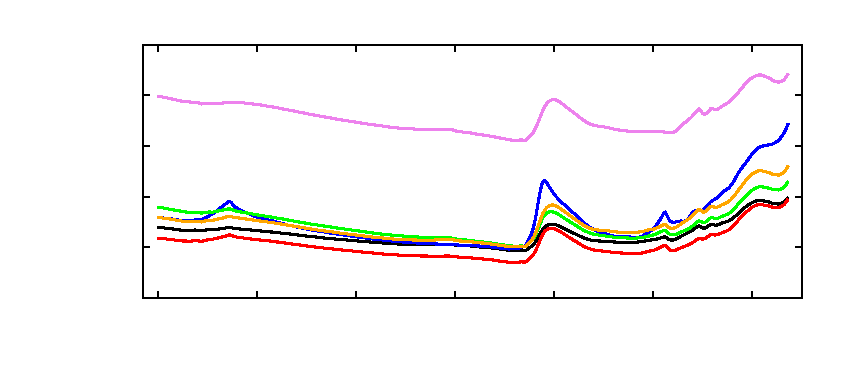
\includegraphics{gp/soil-spec-rnd}}%
    \gplfronttext
  \end{picture}%
\endgroup

			\caption{Six near infrared soil spectra of randomly chosen soil samples obtained from the data set, where $\lambda$ is the wavelength and $\rho(\lambda)$ the corresponding reflectance and each colour refers to one sample}
			\label{fig:soil-spec-rnd}
		\end{figure*}
		
	
	% subsection measured-data

	\subsection{Statistical Model}
	\label{ssec:statistical-model}
	
		Let $n\in\SN$ be the size of the data set and $k\in\SN$ with $k< n$ the number of measured wavelengths. We define
		$\varrho_i$ as the soil spectrum of the $i$th sample for every $i\in\SN,i\leq n$.
		$\lambda_j$ is the $j$th measured wavelength for every $j\in\SN,j\leq k$. We will alternatively refer to these as predictors.
		Then according to section \ref{ssec:measured-data} the measured reflectance values are $x_{ij}$ with
		\[
			x_{ij} \define -\lg \varrho_i(\lambda_j)
		\]
		for every $i,j\in\SN,i\leq n,j\leq k$.
		
	
		We define the measured ASF of $\m{SOC}$ of the $i$th sample for every $i\in\SN,i\leq n$ as $p^\m{(SOC)}_i$ to which we will also refer to as response variable.
		To simplify notation, we then define the $n$-dimensional vector
		\[
			p^\m{(SOC)} \define \curvb{p^\m{(SOC)}_i}
		\]

		The Beer-Lambert law allows us to make assumptions on the relations between soil spectra and the response variable \cite[247-8, 254]{agelet:10a}.
		We saw in section \ref{ssec:nirs} that the logarithmised reflectance can be written as a linear combination of molar concentrations.
		Hence, it seems plausible to assume that an ASF can be represented by a linear combination of logarithmised reflectance values.

		Now let $P^\m{(SOC)}$ be the appropriate random vector to $p^\m{(SOC)}$.
		Then under the above assumption the expected values are given for all $i \in \SN, i \leq n$ by
		\[
			\expect P_i^\m{(SOC)} \define \beta^\m{(SOC)}_0 + \sum_{j = 1}^k{x_{ij}\beta^\m{(SOC)}_j} 
		\]
		which simplifies with an $\mathbb{X} \in \SR^{n \times (k+1)}$, called design matrix, and a parameter vector $\beta^\m{(SOC)} \in \SR^{k+1}$ to
		\[
			\expect P^\m{(SOC)} = \mathbb{X}\beta^\m{(SOC)}
		\]
		
		To capture the stochastic part of $P^\m{(SOC)}$, we extend the model to
		\begin{alignat*}{3}
			&P^\m{(SOC)} = \mathbb{X}\beta^\m{(SOC)} + \varepsilon^\m{(SOC)} \\
			&\expect \varepsilon^\m{(SOC)} = 0, \qquad \cov \varepsilon^\m{(SOC)} = (\sigma^2)^\m{(SOC)} \idmat
		\end{alignat*}
		where $(\sigma^2)^\m{(SOC)} \in (0,\infty)$. Following common practice in physics and chemistry, we further assume that 
		\[
			\varepsilon^\m{(SOC)} \sim \FN \curvb{0,(\sigma^2)^\m{(SOC)}\idmat}
		\]
		This results in the complete model
		\[
			P^\m{(SOC)} \sim \FN \curvb{\mathbb{X}\beta^\m{(SOC)},(\sigma^2)^\m{(SOC)} \idmat}
		\]
		The model for the second response variable $P^\m{(N)}$ is constructed in analogy.
		
		The case for the $\m{pH}$ is slightly different, though. 
		When modelling the corresponding random variable we have to adjust the model as the $\m{pH}$ is a logarithmised molar concentration.
		We therefore have to include this into the expected value of the corresponding random variables
		
		\[
			\expect \m{\overline{pH}}_i \define \beta^\m{\m{(pH)}}_0 + \sum_{j = 1}^k{\ln (x_{ij}) \beta^\m{(pH)}_j} 
		\]
		and denote the corresponding matrix by $\mathbb{X}_{\ln}$.

	
	% subsection statistical-model

	\subsection{Multivariate Linear Regression}
	\label{ssec:mlr}
	
		Multivariate linear regression (MLR) is a statistical method for estimating parameters of linear relations between a response variable and a set of predictors.
		These can be reused to predict new responses \cite{draper:98a, pardoe:12a, schumacher:16a}.
		Let $\mathbb{X}\in\SR^{n\times(k+1)}, n,k\in\SN,k<n$ be the design matrix with $\rank{\mathbb{X}} = k+1$, $\sigma^2\in(0,\infty)$ and $Y$ be the random vector of a response variable with
		\[
			Y \sim \FN\curvb{\mathbb{X}\beta,\sigma^2\idmat_n}
		\]
		for a certain $\beta\in\SR^{k+1}$.
		Then through the maximum-likelihood-method and a correction we get two best unbiased estimators $\hat{\beta},\hat{\sigma}^2$ for $\beta$ and $\sigma^2$
		\begin{alignat*}{3}
			\hat{\beta}(Y) &=&&\ \inv{\curvb{\transp{\mathbb{X}}\mathbb{X}}}\transp{\mathbb{X}}Y \\
			\hat{\sigma}^2(Y) &=&&\ \frac{1}{n-(k+1)}\norm{Y - \mathbb{X}\hat{\beta}(Y)}^2
		\end{alignat*}
		Now let $y \define (y_i)\in\SR^n$ be a realization of $Y$.
		Then we define
		\begin{alignat*}{3}
			\hat{y} &\define&&\ \mathbb{X}\hat{\beta}(y) = \mathbb{X}\inv{\curvb{\transp{\mathbb{X}}\mathbb{X}}}\transp{\mathbb{X}}y \\
			\tilde{\sigma}^2 &\define&&\ \hat{\sigma}^2(y)
		\end{alignat*}

	% subsection mlr

	\subsection{Mallows' $C_\m{p}$}
	\label{ssec:mallows-C_p}
	
		At this point, the model is specified using $k+1 = 320$ predictors for each response variable, using the whole domain of measured spectrum for each soil sample.
		This set of predictors is comparatively large, $n-k < k$.
		Further, the reflectances of neighbouring lightwaves are correlated \cite[252]{agelet:10a}.
		In these circumstances, we might overfit the data, i.e. the variance of our estimated parameters $\hat{\beta}_i(Y)$ might be too large, compromising their usability for future measurements.
		To address this problem, it is sensible to limit each actual model to a \enquote{good} subset of the predictors. Hence, our task transform into selecting the best or at least a \enquote{sufficiently} good model $M$ defined by
		\[
			M\subset \Lambda \cup \set{\lambda_0} \definedby \overline{\Lambda}
		\]
		where $\lambda_0$ stands for the intercept.
		We denote the design matrix for each $M$ by $\mathbb{X}^{(M)}$.
		Applying MLR to the new design matrix yields the new estimators
		\begin{alignat*}{3}
			\hat{\beta}^{(M)}(Y) &=&&\ \inv{\curvb{\transp{\mathbb{X}^{(M)}}\mathbb{X}^{(M)}}}\transp{\mathbb{X}^{(M)}}Y \\
			\curvb{\hat{\sigma}^2}^{(M)}(Y) &=&&\ \frac{1}{n-\m{p}}\norm{Y - \mathbb{X}^{(M)}\hat{\beta}^{(M)}(Y)}^2_2,
		\end{alignat*}
		where $\m{p} \in \set{1,\ldots,k+1}$ corresponds to the number of predictors included in $M$.
		
		The sum of predicted squared errors ($\m{SPSE}$) is a theoretical criterion to compare the merits of different models.
		The $\m{SPSE}$ measures how well a model does in predicting new responses for new observations $Y_{n+i}$ which are iid to $Y_i$ for $i \in \SN, i \leq n$ and is given by
		\[
			\m{SPSE}^{(M)} \define \sum_{i = 1}^n \expect \curvb{Y_{n+i} - \hat{Y}_i^{(M)}}^2
		\]
		which simplifies to \cite[29-30]{schumacher:16a}
		\[
			\m{SPSE}^{(M)} = n\sigma^2 + \m{p}\sigma^2 + \curvb{\m{bias}^2}^{(M)}
		\]
		where $\m{bias}$ describes the divergence of the estimated expectation from the true expectation.
		As $\m{bias}$ is decreasing in the number of parameters included in $M$, we assume it to be sufficiently close to zero to neglect it from further considerations \cite{schumacher:16b}.
		
		Unfortunately, the true $\sigma^2$ is unobservable so that it has to be estimated by
		\[
			\widehat{\m{SPSE}}^{(M)}(Y) \define \norm{Y - \mathbb{X}^{(M)}\hat{\beta}^{(M)}(Y)}^2_2 + 2\m{p}\hat{\sigma}^2(Y)
		\]
		
		Instead of using the $\widehat{\m{SPSE}}^{(M)}$ directly, we will use Mallow's $C_\m{p}$ instead, given by
		\[
			C_\m{p}^{(M)} \define \frac{1}{\tilde{\sigma}^2}\sum_{i=1}^n\curvb{y_i-\hat{y}^{(M)}_i}^2 - n + 2\m{p}
		\]
		Minimising this value is equivalent to the minimisation of the $\widehat{\m{SPSE}}^{(M)}$.
		% The proof is trivial, just biject it to a conext-free residue class, whose elements are open manifolds. %citation
	
	% subsection mallows-C_p

	\subsection{Simulated Annealing}
	\label{ssec:model-selec}
	
		We can now formulate the following minimisation problem.
		Let
		\[
			\s{H} \define \set[A\in\setpow(\Lambda)]{A \cup \set{\lambda_0}} \subset \setpow\curvb{\overline{\Lambda}}
		\]
		Then the model we want to select is a solution to
%		\[
%			\curvb{\Omega} \qquad \minimize_{M\in\s{H}} \qquad C_\m{p}^{(M)}
%		\]
		\[
			\Omega \define \minimize \; \set[M\in\s{H}]{C_\m{p}^{(M)}}
		\]
		This problem is a discrete optimisation problem, which is in general np-hard \cite[245-50]{schrijver:98a}.
		Unfortunately, $\abs{\s{H}} = 2^{319}$, which is too large for a complete search.
		Therefore, we need a heuristic search algorithm that does not depend on further information of the cost function.

		Simulated annealing (SANN) is such an algorithm that approximates global optima of a given function \cite[549-54]{press:07a}.
		Note that the SANN returns only a probabilistically good approximation $\s{M}\in\s{H}$ to a true solution to $\Omega$.
		Lacking similarly reliable and computationally feasible alternatives we use the solution returned by SANN instead.

		The algorithm is applicable to arbitrary sets, in our case $\s{H}$.
		It simulates the slow cooling of a thermodynamic system.
		Let $x_0\in\s{H}$ be the initial set of predictors, $T_0\in(0,\infty)$ be the initial temperature of the system and $i_\m{max}\in\SN$ be the maximal number of time steps.
		Then the algorithm requires the following functions:
		\begin{itemize}
			\item $\func{\m{cost}}{\s{H}}{\SR}$ \\
				Calculates the cost of a given predictor set.
			\item $\func{\m{temp}}{\SR\times\SN^2}{(0,\infty)}$\\
				Calculates the temperature according to the given initial temperature and time steps.
				It is a monotonically decreasing function in the second parameter.
			\item $\func{\m{nbr}}{\s{H}}{\s{H}}$ \\
				Generates a random neighbour of a given predictor set.
			\item $\func{\m{prob}}{\SR^2\times(0,\infty)}{[0,1]}$ \\
				Calculates the probability of changing the current set or state to the neighbour.
			\item $\m{rnd}(0,1)$ \\
				Returns a random number in the interval $[0,1]$.
		\end{itemize}
		The listing shows one variant of the pseudocode of the SANN algorithm. 

		\medskip
		\begin{tcolorbox}[colframe=black,colbacktitle=white,coltitle=black, attach boxed title to top center={yshift=-2mm},enhanced, titlerule=0.1pt, boxrule=0.5pt, arc=5pt,title=Listing:\quad SANN algorithm]
			\begin{tabbing}
	\qquad\=\qquad\=\qquad\=\qquad\=\kill
	$c_0 = \m{cost}(x_0)$\\
	\\
	\textbf{for} ($i=1$, $i\leq i_\m{max}$) \{\\
		\>$T = \m{temp}(T_0,i,i_\m{max})$\\
		\\
		\>$x_1 = \m{nbr}(x_0)$\\
		\>$c_1 = \m{cost}(x_1)$\\
		\\
		\>\textbf{if} $(\m{prob}(c_0, c_1, T) \geq \m{rnd}(0,1))$ \{\\
			\>\>$x_0 = x_1$\\
			\>\>$c_0 = c_1$\\
		\>\}\\
	\}
\end{tabbing}
		\end{tcolorbox}
		\medskip

	% subsection simulated-annealing
		
	\subsection{Model Validation}
	\label{ssec:model-validation}
	
		To examine the models selected by SANN, we recur to the often used $R^2$ measure \cite[33-4]{draper:98a}.
		For $M\in\s{H}$ it is given by
		\[
			\curvb{R^2}^{(M)} \define \frac {\sum_{i=1}^n \curvb{\hat{y}^{(M)}_i - \overline{y}}^2}{\sum_{i=1}^n \curvb{y_i - \overline{y}}^2} \in [0,1]
		\]
		where $\overline{y}$ is the arithmetic mean of $y_i$ for $i=1,\ldots,n$ and describes how much of the total variation of $y$ is explained by the model $M$.
		$\curvb{R^2}^{(M)} = 0$ is equivalent to no, $\curvb{R^2}^{(M)} = 1$ to full agreement of the model with the observations.
		
		We shall note though, that the measure is increasing with $\abs{M}$.
		In contrast the actual upper bound of $R^2$ is lowered by the presence of measurement errors.
		We will therefore consult the correlation diagrams for each response variable observation vector and its respective prediction vector to complement our judgement based on the $R^2$ measure alone.

	% subsection model-validation
	
	\subsection{Assessment by Simulation}
	\label{ssec:simulation}
	
		As the true $\m{SPSE}$ is unobservable, we need to assess how well our procedure minimises the true $\m{SPSE}$ in general.
		For limitations of available data we have to resort to so called pseudo-observations of a response variable, which we collect in a random vector as follows
		\[
			\widetilde{Y} \define \hat{y}^{(\s{M})} + \varepsilon,\qquad \varepsilon \sim  \FN \curvb{0,\sigma^2\idmat_n}
		\]
		where we assign
		\[
			\sigma^2 \define \curvb{\tilde{\sigma}^2}^{(\s{M})}
		\]
		Having fixed the parameters for the random vector $\widetilde{Y}$ we can now calculate the true $\m{SPSE}$ from them by
		\[
			\m{SPSE}^{(\s{M})} = \curvb{ n + \abs{\s{M}} } \sigma^2
		\]
		
		We can now simulate a new application of our model selection algorithm for
		\[
			\widetilde{Y} \sim \FN\curvb{\mathbb{X}\widetilde{\beta},\sigma^2\idmat_n}
		\]
		treating $\sigma^2$ as unknown.
		The algorithm returns a model $\widetilde{\s{M}}$. We can now calculate $\widehat{\m{SPSE}}^{(\widetilde{\s{M}})}$ and compare it to the true $\m{SPSE}$.
		Due to the heuristic nature of the selection algorithm, we might end up with an exceptionally bad value.
		To address this, we repeat this process $q\in\SN$ times \cite{schumacher:16b}.
		
		In addition to parameters of the random vector $\widetilde{Y}$, $\widehat{\m{SPSE}}^{(\widetilde{\s{M}})}$ depends on the hyperparameters, resolution $k = \abs{\Lambda}$ and the number of observations, $n$, as well.
		To gauge influences of the resolution on the model selection, we augment the procedure above to include the sets
		\[
			\Lambda^{(m)} \define \set[i\in\SN, m \cdot i \leq k]{\lambda_{m\cdot i} \in \Lambda}
		\]
		where $m \in \set{1, 2, 3, 4}$ and $\Lambda^{(m)}$ takes replace of $\Lambda$ in \ref{ssec:mallows-C_p} and \ref{ssec:model-selec}.
		
		To assess the influence of the number of available measurements, we choose randomly selected subsets of the existing measurements of sizes $n \in \set{100, 200, 300, 500, 533}$ and augment the simulation accordingly.
		In this way, we can compare the $\widehat{\m{SPSE}}^{(\widetilde{\s{M}})}$ with the \enquote{true} model's $\m{SPSE}$ in 19 situations and on the same $r$ pseudo-observations for each.
		
	% subsection simulation
% section methodology